\documentclass{llncs}
\usepackage{amsmath,amssymb,calc,ifthen}
\usepackage{float}
%\usepackage{cancel}
\usepackage[table,usenames,dvipsnames]{xcolor} % for coloured cells in tables
\usepackage{tikz}
% Allows us to click on links and references!
\usepackage{hyperref}
\usepackage{url}
\hypersetup{
colorlinks,
citecolor=black,
filecolor=black,
linkcolor=black,
urlcolor=black
}
% Nice package for plotting graphs
% See excellent guide:
% http://www.tug.org/TUGboat/tb31-1/tb97wright-pgfplots.pdf
\usetikzlibrary{plotmarks,shapes}
\usepackage{amsmath,graphicx}
\usepackage{epstopdf}
\usepackage{caption}
\usepackage{subcaption}
\usepackage{graphicx}
% highlight - useful for TODOs and similar
\usepackage{color}
\newcommand{\hilight}[1]{\colorbox{yellow}{#1}}
\newcommand\ci{\perp\!\!\!\perp} % perpendicular sign
\newcommand*\rfrac[2]{{}^{#1}\!/_{#2}} % diagonal fraction
\newcommand\SLASH{\char`\\}
\usepackage{listings}
% margin size
\usepackage{pdfpages}
\usepackage{enumitem} % for nested enumerate numbers 1 1.1 1.1.1
% \usepackage{breqn}
% \usepackage[linesnumbered]{algorithm2e}
% \usepackage{algorithmicx,algpseudocode}
% \usepackage{wrapfig} % for allowing text wrapped around the algorithm
% \newcommand\mycommfont[1]{\footnotesize\ttfamily\textcolor{blue}{#1}}
% \SetCommentSty{mycommfont}

% \usepackage{titlesec}
% \titlespacing*{\section}
% {0pt}{5.5ex plus 1ex minus .2ex}{4.3ex plus .2ex}


\DeclareMathOperator*{\argmin}{arg\,min}
\DeclareMathOperator*{\argmax}{arg\,max}

\begin{document}

\definecolor{blue3}{HTML}{86B7FC} % med blue
\definecolor{blue1}{HTML}{B5F1FF} % light blue
\definecolor{blue2}{HTML}{E0F9FF} % very light blue

\title{A vertex clustering model for disease progression: Application to cortical thickness images}
%
\titlerunning{Vertex clustering model for disease progression}  % abbreviated title (for running head)
%                                     also used for the TOC unless
%                                     \toctitle is used
%
\author{R\u{a}zvan V. Marinescu\inst{1} \and Arman Eshaghi\inst{1,2} \and
Marco Lorenzi\inst{1,4} \and Alexandra L. Young\inst{1} \and Neil P. Oxtoby\inst{1} \and Sara Garbarino\inst{1} \and Timothy J. Shakespeare\inst{3} \and Sebastian J. Crutch\inst{3} \and Daniel C. Alexander\inst{1}, for 
the  Alzheimer’s  Disease  Neuroimaging Initiative\thanks{Data used in preparation of this article were obtained from the Alzheimer's Disease Neuroimaging Initiative (ADNI) database (adni.loni.usc.edu). As such, the investigators within the ADNI contributed to the design and implementation of ADNI and/or provided data but did not participate in analysis or writing of this report. A complete listing of ADNI investigators can be found at: http://adni.loni.usc.edu/wp-content/uploads/how\_to\_apply/ADNI\_Acknowledgement\_List.pdf}}

%
\authorrunning{R\u{a}zvan V. Marinescu et al.} % abbreviated author list (for running head)
%
%%%% list of authors for the TOC (use if author list has to be modified)
% \tocauthor{Ivar Ekeland, Roger Temam, Jeffrey Dean, David Grove,
% Craig Chambers, Kim B. Bruce, and Elisa Bertino}
%
\institute{Centre for Medical Image Computing, Computer Science Department, University College London, UK
\and 
Queen Square MS Centre, UCL Institute of Neurology, London
\and 
Dementia Research Centre, UCL Institute of Neurology, University College London, UK
\and
University of C\^{o}te d'Azur, Inria Sophia Antipolis, Asclepios Research Project
% Laboratoire d'Analyse Num\'{e}rique, B\^{a}timent 425,\\
% F-91405 Orsay Cedex, France}
}

\maketitle              % typeset the title of the contribution

\begin{abstract}
% The abstract should summarize the contents of the paper
% using at least 70 and at most 150 words. It will be set in 9-point
% font size and be inset 1.0 cm from the right and left margins.
% There will be two blank lines before and after the Abstract. \dots

%5. achievement: we built a voxelwise disease progression model that uses sigmoidal traj
%6. model groups together vertices into clusters and builds a common trajectory for all vertices in the cluster
%7. Simulations show bla bla ...
%8. Tested the model on ADNI and stages correlate well with cognitive tests.
%9. Compared the patterns of typical and atypical AD with DRC data

% The model highlights, for the first time, groups of brain vertices that exhibit a similar temporal trajectory over the population. This provides a new way to parcellate the brain that is specific to the temporal trajectory of a particular disease

%%% MAX NR OF WORDS USED, DO NOT ADD MORE %%%%%%

We present a disease progression model with single vertex resolution that we apply to cortical thickness data. Our model works by clustering together vertices on the cortex that have similar temporal dynamics and building a common trajectory for vertices in the same cluster. The model estimates optimal stages and progression speeds for every subject. Simulated data show that it is able to accurately recover the vertex clusters and the underlying parameters. Moreover, our clustering model finds similar patterns of atrophy for typical Alzheimer's disease (tAD) subjects on two independent datasets: the Alzheimer's Disease Neuroimaging Initiative (ADNI) and a cohort from the Dementia Research Centre (DRC), UK. Using a separate set of subjects with Posterior Cortical Atrophy (PCA) from the DRC dataset, we also show that the model finds different patterns of atrophy in PCA compared to tAD. Finally, our model provides a novel way to parcellate the brain based on disease dynamics.


\keywords{Disease Progression Model, Cortical Thickness, Vertex-wise Measures, Alzheimer's Disease, Posterior Cortical Atrophy}
\end{abstract}

%%%%%%%%% NO LONGER THAN 12 pages!! otherwise paper will be instantly rejected %%%%%%%%

\section{Introduction}

% Modelling progression of neurodegenerative diseases such as
% Alzheimer’s disease is difficult because only short-term followup data is
% available and because subjects are at di↵erent stages of the disease. Previous
% disease progression models have been used to solve this complex
% problem, but MRI biomarkers that were used such as cortical thickness
% were averaged across regions of interest (ROI). This can be problematic,
% especially if di↵erent parts of the ROI, say hippocampus, is a↵ected at
% di↵erent speeds or timepoints in the disease process. A vertexwise disease
% progression model has been recently proposed to mitigate this problem,
% but it assumes biomarker trajectories are linear in order to make the
% fitting process tractable.

% grand challenge in disease progression modelling
During the progression of Alzheimer's disease, many biomarkers based on Magnetic Resonance Imaging (MRI) such as cortical thickness become abnormal at different points in the progression. Finding out the precise temporal evolution of these biomarkers facilitates patient staging in clinical trials. However, the analysis of disease progression is limited by several factors: short number of follow-up visits available, different disease onset and progression speed for every subject and cohort heterogeneity. 

% hypothetical models + models that require a priori clinical categories
A hypothetical model of disease progression has been proposed by \cite{jack2010hypothetical}, describing the trajectory of key biomarkers along the progression of Alzheimer's disease. The model suggests that amyloid-beta and tau biomarkers become abnormal long before symptoms appear, followed by brain atrophy measures and cognitive decline. Motivated by this idea, several models such as \cite{bateman2012clinical} or \cite{richberg2015multi} have been proposed that reconstruct biomarker trajectories and can be used to stage subjects. However, these models make use of \emph{a priori} clinical categories, which are noisy, biased and can limit the temporal resolution of the model. This motivates the use of fully data-driven approaches that do not use \emph{a priori} clinical stages. 

% models that estimate trajectories of a small set of biomk
Various data-driven disease progression modelling techniques have been proposed in recent years. One such model is the Event-Based Model \cite{fonteijn2012event}, which models the progression of disease as a sequence of discrete events, representing underlying biomarkers switching from a normal to abnormal state. Other models such as the Disease Progression Score (DPS) \cite{jedynak2012} or self-modelling regression approaches \cite{donohue2014estimating} have been developed, that build continuous trajectories by "stitching" together short-term follow-up data. Models estimating linear or logistic trajectories by means of Riemannian manifold techniques have also been recently shown \cite{schiratti2015mixed}.

% motivate the idea of avoiding a priori region specification
The main limitation of these data-driven models is that they use a small set of biomarkers that are obtained by averaging MRI or PET measures across all voxels or vertices in a Region of Interest (ROI). This can be problematic, especially if different parts of the ROI, say the hippocampus, are affected at different speeds or timepoints in the disease process. Therefore, moving to a voxel-wise approach would allow one to estimate the fine-grained spatial distribution of atrophy, which could give new insights into the disease process and potentially enable more precise staging. A voxel-wise disease progression model \cite{bilgel2016multivariate} has been recently proposed to mitigate this problem, that uses amyloid measures in each voxel as its input data. However, the model by \cite{bilgel2016multivariate} has two limitations: (1) the biomarker trajectories are assumed to be linear, so cannot capture the plateau effect observed in amyloid-beta or tau and (2) the model uses a spatial correlation function for modelling correlation between voxels; while this is necessary, due to the nature of the imaging data, it has been shown that in different types of dementia atrophy patterns match functional networks, which are not spatially connected \cite{seeley2009neurodegenerative}.

% Present my work
In this work, we present a new disease progression model with single vertex resolution that avoids assumptions on spatial correlation. We combine unsupervised learning and disease progression modelling to identify clusters of vertices on the cortical surface, with no spatial constraints, that show a similar trajectory of atrophy over a particular patient cohort. This formulation enables us to gain new insights into the spatial structure of atrophy in different diseases and also provides a novel parcellation of the brain based on temporal change. Moreover, each cluster of vertices has a corresponding sigmoidal trajectory, which avoids the limitation of linear trajectories in \cite{bilgel2016multivariate}. 

% Mention briefly what has been achieved so far
We first show using simulated data that our model is able to recover known underlying clusters, trajectory parameters and subject stages. We then apply our model to cortical thickness vertex-wise measures using ADNI and the DRC dataset and highlight the new insights the model can give. Finally, we validate our model using cross-validation and by correlating the subject stages with cognitive measures.

% We first show that our algorithm gives similar answers on the two independent typical AD datasets (ADNI and DRC datasets). Secondly, when modelling distincts disease populations (PCA vs AD), our method finds different atrophy patterns which broadly reflect the known spatial distribution of atrophy in each condition. Finally, using cross calidation on the ADNI data we show that the model is robustly recovering the same clusters and that the stages are clinically meaningful, as they correlate with four different cognitive tests.

\section{Methods}

\subsection{Model}

% progresison score, affine transformation
We seek to identify groups of image vertices that show a common trajectory during the disease course, while simultaneously placing each visit from each subject within that disease course. In a similar way to \cite{jedynak2012,donohue2014estimating,schiratti2015mixed}, we estimate a time shift and speed (or rate) of progression for each subject. We relate these time shifts and progression speeds by assigning each subject a disease stage which we will refer to as the Disease Progression Score (DPS). In contrast to \cite{jedynak2012,donohue2014estimating,schiratti2015mixed}, which model temporal trajectories for a small set of biomarker measures based on \emph{a priori} defined ROIs, we model temporal trajectories for each vertex on the cortical surface. Each trajectory is a function of the disease progression score (i.e. disease stage) of a subject. We estimate each subjects' time shift, progression speed and trajectory parameters from the data. The disease progression score $s_{ij}$ for subject $i$ at visit $j$ is defined as a linear transformation of age $t_{ij}$:

\begin{equation}
\label{eq:dps}
 s_{ij} = \alpha_i t_{ij} + \beta_i
\end{equation}
% sigmoidal functions
where $\alpha_i$ and $\beta_i$ represent the speed of progression and time shift (i.e. disease onset) of subject $i$. 

Our model assumes that the cortical thickness at each vertex on the cortical surface follows a sigmoidal trajectory $f(s)$ given the disease progression score $s$. We also assume that vertices are grouped into $K$ clusters and we model a unique trajectory for each cluster $k \in [1, \dots, K]$, which will be referred to as cluster trajectories. The sigmoidal function for cluster $k$ is parametrised as $\theta_k = [a_k,b_k,c_k,d_k]$ where 

\begin{equation}
 f(s;\theta_k) = \frac{a_k}{1+exp(-b_k(s-c_k))} + d_k
\end{equation}

For a given subject $i$ at visit $j$, the value $V_l^{ij}$ of its cortical thickness at vertex $l$ is a random variable that has an associated discrete latent variable $Z_l \in [1, \dots, K]$ denoting the cluster it was generated from. The value of $V_l^{ij}$ given that it was generated from cluster $Z_l$ can be modelled as:

% TODO cannot use Z_l for the index of theta and for a random variable, use smth like Z_l = z_l, but watch out later on not to have conflicts.

% model for one voxel and label
\begin{equation}
 p(V_l^{ij} | \alpha_i, \beta_i, \theta_{Z_l}, \sigma_{Z_l}, Z_l) = N(V_l^{ij} | f(\alpha_i t_{ij} + \beta_i | \theta_{Z_l}), \sigma_{Z_l})
\end{equation}
where $N(V_l^{ij} | f(\alpha_i t_{ij} + \beta_i | \theta_{Z_l}), \sigma_{Z_l})$ represents the pdf of the normal distribution that models the measurement noise along the sigmoidal trajectory of cluster $Z_l$, having variance $\sigma_{Z_l}$. Next, we assume the measurements from different subjects are independent, while the measurements from the same subject $i$ at different visits $j$ are linked using the disease progression score from equation \ref{eq:dps}, because we estimate only two parameters ($\alpha_i$ and $\beta_i$) using the data from all visits $j$. Moreover, we also assume a uniform prior on $Z_l$. This gives the following model:

% all subj are independent
\begin{equation}
 p(V_l, Z_l | \alpha, \beta, \theta, \sigma) = \prod_{(i,j) \in I} N(V_l^{ij} | f(\alpha_i t_{ij} + \beta_i | \theta_{Z_l}), \sigma_{Z_l})
\end{equation}
where $I = {(i,j)}$ represents the set of all the subjects $i$ and their corresponding visits $j$. Furthermore, $V_l = [V_l^{ij} | (i,j) \in I]$ is the 1D array of all the values for vertex $l$ across every subject and corresponding visit. Vectors $\alpha = [\alpha_1, \dots, \alpha_S]$ and $\beta = [\beta_1, \dots, \beta_S]$, where $S$ is the number of subjects, denote the stacked parameters for the subject shifts. Vectors $\theta = [\theta_1, \dots, \theta_K]$ and $\sigma = [\sigma_1, \dots, \sigma_K]$, with $K$ being the number of clusters, represent the stacked parameters for the sigmoidal trajectories and measurement noise specific to each cluster.

We further assume all vertex measurements to be spatially independent, giving the complete data likelihood:

% all vertices are independent
\begin{equation}
 p(V, Z | \alpha, \beta, \theta, \sigma) = \prod_l^L \prod_{(i,j) \in I} N(V_l^{ij} | f(\alpha_i t_{ij} + \beta_i | \theta_{Z_l}), \sigma_{Z_l})
\end{equation}
where $V = [V_1, \dots, V_L]$, $Z = [Z_1, \dots, Z_L]$, $L$ being the total number of vertices on the cortical surface. We recall that we don't want to enforce spatial correlation between vertices as we are interested to see if vertices from distinct areas of the brain are grouped together in the same cluster. Our assumption is also justified by the fact that we smoothed the cortical thickness images in the preprocessing steps. We get the final model log likelihood for incomplete data by marginalising over the latent variables $Z$:
\begin{equation}
 p(V|\alpha, \beta, \theta, \sigma) = \prod_{l=1}^L \sum_{k=1}^K p(Z_l = k) \prod_{(i,j) \in I} N(V_l^{ij} | f(\alpha_i t_{ij} + \beta_i | \theta_k), \sigma_k)
\end{equation}
Therefore, the parameters that need to be estimated are $\Theta = [\alpha, \beta, \theta, \sigma]$ where $\alpha$ and $\beta$ are the subject specific shifting parameters while $\theta$ and $\sigma$ are the cluster specific trajectory and noise parameters. 

\subsection{Fitting the Model using EM}

Due to the summing over the latent variables $Z$, it is not possible to find a closed form solution to the maximum likelihood. Therefore, we fit our model using Expectation-Maximisation, which is suitable given the large number of data points and parameters that need to be estimated. 

% We therefore seek to maximize:
% \begin{equation}
% \label{eq:EMgen}
% \argmax_{\Theta} E_{Z|V,\Theta^{old}} [log\ p(V,Z|\Theta)] + log\ p(\Theta) 
% \end{equation}
% where $\Theta^{old} = (\alpha^{old}, \beta^{old}, \theta^{old}, \sigma^{old})$ and $log\ p(\Theta)$ is a prior on the parameters.

\subsubsection{E-step}

In the Expectation step we seek to estimate which cluster has generated each of the $L$ vertices, given the current estimates of the cluster parameters $\theta_k^{old}, \sigma_k^{old}$ as well as the subject specific shift parameters $\alpha_i^{old}, \beta_i^{old}$. More formally, we seek to find $p(Z|V,\Theta^{old}) = \prod_l^L p(Z_l|V_l,\Theta^{old})$, given our independence assumption between vertices. Let us denote by $z_{lk} = p(Z_l = k | V_l,\Theta^{old})$. We then have:

\begin{equation}
 z_{lk} =  \frac{\prod_{(i,j) \in I} N(V_l^{ij} | f(\alpha_i^{old} t_{ij} + \beta_i^{old} | \theta_k^{old}), \sigma_k^{old})}{\sum_{m=1}^K \prod_{i,j \in I} N(V_l^{ij} | f(\alpha_i^{old} t_{ij} + \beta_i^{old} | \theta_m^{old}), \sigma_m^{old})}
\end{equation}
Ignoring the normalisation factor, we perform a log transformation and expand the pdfs of the normal distributions. This results in the following update equation for the E-step:

\begin{equation}
 log\ z_{lk} \propto  -\frac{1}{2} log\ (2 \pi \left(\sigma_k^{old}\right)^2) |I| - \frac{1}{2\left(\sigma_k^{old}\right)^2} \sum_{(i,j) \in I} (V_l^{ij} - f(\alpha_i^{old} t_{ij} + \beta_i^{old} | \theta_k^{old}))^2 
\end{equation}
The original probabilities can be easily recovered by exponentiating them and then normalising with respect to their sum.

\subsubsection{M-step}

In the Maximisation step we try to find $\Theta = (\alpha, \beta, \theta, \sigma)$ that maximise $E_{Z|V,\Theta^{old}} [log\ p(V,Z|\Theta)]$. Since there is no closed-form solution, we perform successive refinements of $\theta_k$ for each cluster $k$ and $\alpha_i, \beta_i$ for each subject $i$ until convergence. 

In order to get the update rule for the trajectory parameters $\theta_k$ corresponding to cluster $k$ we need to maximise the expected log likelihood with respect to $\theta_k$. We get the following simplified optimisation problem:

\begin{equation}
 \label{eq:theta}
 \theta_k = \argmin_{\theta_k} \left[\sum_{l=1}^L z_{lk} \sum_{(i,j) \in I} (V_l^{ij} - f(\alpha_i t_{ij} + \beta_i | \theta_k))^2 \right] - log\ p(\theta_k) 
\end{equation}
A similar equation is also obtained for $\sigma_k$. After estimating $\theta$ and $\sigma$ for every cluster, we use the new values to estimate the subject specific parameters $\alpha$ and $\beta$. Let $S$ be the number of subjects and $\alpha_i$, $\beta_i$ be the rate and shift for subject $i \in S$. We again maximise the expected log likelihood with respect to $\alpha_i$, $\beta_i$ independently, and after simplifications we obtain the following problem:

\begin{equation}
\label{eq:alpha}
 \alpha_i, \beta_i = \argmin_{\alpha_i, \beta_i}  \left[ \sum_{l=1}^L \sum_{k=1}^K z_{lk} \frac{1}{2\sigma_k^2} \sum_{j \in I_i} (V_l^{ij} - f(\alpha_i t_{ij} + \beta_i | \theta_k))^2\right] - log\ p(\alpha_i, \beta_i)
\end{equation}

In summary, at every single M-step, we iterate between solving for $\theta$, $\sigma$ and solving for $\alpha$, $\beta$ using numerical optimisation until convergence. Due to the use of numerical optimisation, we are not guaranteed to find the global maxima for the expected log likelihood, but EM still works if we only find an increase in the log-likelihood. This approach that involves a partial M-step is called Generalised EM.

\subsection{Initialisation and Implementation}
\label{sec:initialisation}
% initialisation
Before starting the fitting process, we need to initialise $\alpha$, $\beta$ and the clustering probabilities $z_{lk}$. We set $\alpha_i$ and $\beta_i$ to be 1 and 0 respectively for each subject. We initialise $z_{lk}$ using k-means clustering using vectors $V_l$ having $|I|$ number of samples and $L$ features. Furthermore, as already explained in \cite{jedynak2012}, the scale of the DPS is arbitrary so we standardise the scores at each EM iteration such that the DPS of controls have a mean $\mu_N$ of zero and a standard deviation $\sigma_N$ of 1. This also requires a rescaling of the cluster parameters $\theta_k$.

In our implementation, we run the main EM loop until convergence of the clustering probabilities $z_{lk}$. At each M-step we perform numerical optimisation using the Broyden-Fletcher-Goldfarb-Shanno (BFGS) algorithm that makes use of the first derivative of the objective function. In all datasets analysed, the method converges after maximum 25 EM iterations. 

\section{Simulation Results}

% Data generation
We first tested the model in a toy scenario using synthetic data, which we generated as follows: (1) sampled age and shift parameters from 300 subjects with 4 timepoints (each timepoint 1 year apart), with $t_{i1} \sim U(40,80)$, $\alpha_i \sim N(1, 0.05)$, $\beta_i \sim N(0, 10)$ (2) generated three sigmoids with different center points and slopes (Fig. \ref{fig:synThetaRes}, red lines) (3) generated a random cluster assignment for $L = 1,000$ vertices, i.e. every vertex $l$ was assigned to a cluster $a[l] \in \{1,2,3\}$ (4) sampled a set of $L$ perturbed trajectories $\theta_l$ from each of the original trajectories, one for each vertex (Fig. \ref{fig:synThetaRes}, gray lines) and (5) sampled subject data for every vertex $l$ from its corresponding perturbed trajectory $\theta_l$ with $\sigma_l = 0.5$

% Method
To fit the data we used a uniform prior on the parameters $\theta$ and $\sigma$ and an informative prior on $\alpha$ and $\beta$, with $p(\alpha_i) \sim \Gamma(49,70)$ and $\beta_i \sim N(0,1)$. We also normalised age to have a mean of 0 and standard deviation of 1 and rescaled the DPS and cluster trajectories accordingly. After convergence, we calculated the agreement between the final clustering probabilities and the true clustering assignments as $A = \frac{1}{L}\sum_{l=1}^L p(Z_l = a[l])$. The method also requires us to set the number of clusters \emph{a priori}, so we optimised the number of clusters using the Bayesian Information Criterion (BIC). 

% Results
The BIC analysis correctly predicted three clusters for this synthetic experiment. Using three clusters, we also obtained a clustering agreement of $A = 1.0$. Figure \ref{fig:synThetaRes} shows the original trajectories and the recovered trajectories using our model, plotted against the disease progression score on the x-axis and the vertex value on the y-axis. Moreover, in Fig. \ref{fig:synShiftRes} we plotted the recovered DPS of each subject along with the true DPS. 

% Conclusion
The results show that the model accurately estimated which clusters generated each vertex. Moreover, the recovered trajectories are close to the true trajectories, with some errors for the trajectories corresponding to clusters 1 and 2. The recovered DPS also shows good agreement with the true DPS, with the exception of a few subjects with DPS greater than 2.5. This is explained by the fact that there is not enough signal in that DPS range in terms of trajectory dynamics (i.e. trajectories are mostly flat). The simulation confirms that our model is able to recover the hidden clusters, trajectory parameters and the subject specific parameters. However, more realistic simulations with varying noise levels and numbers of clusters are required to understand the limitations of the model and find out when it fails to recover the true parameters. 


\begin{figure}[h]
\begin{subfigure}[b]{0.75\textwidth}
  \hspace{-2em}
  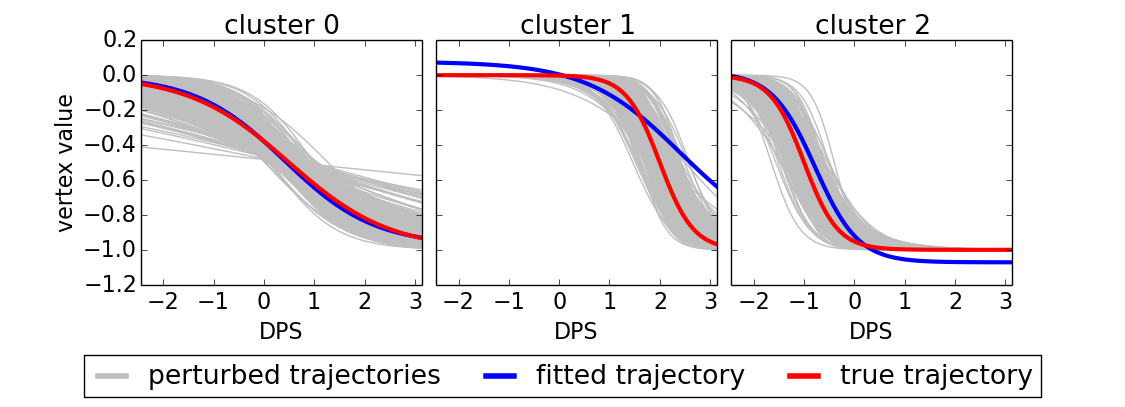
\includegraphics[width=1.15\textwidth,trim=0 10 0 50]{figures//synThetaRes_gensigInitk-meansCl3Pr1Ra0_VWDPMStd.png}
  \caption{}
  \label{fig:synThetaRes}
\end{subfigure}
\hspace{-1em}
\begin{subfigure}[b]{0.24\textwidth}
\centering
  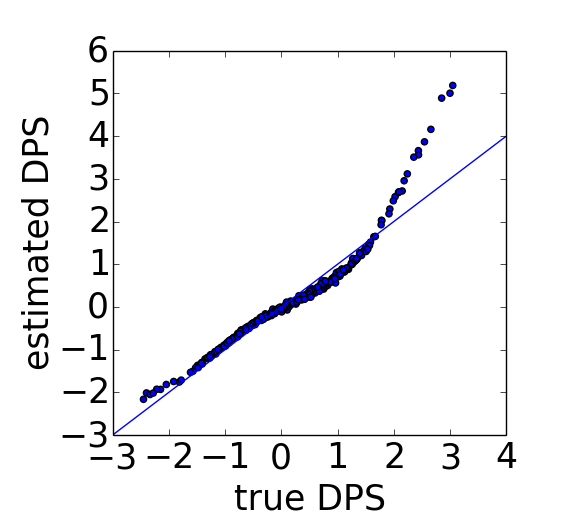
\includegraphics[width=1.2\textwidth,trim=0 20 0 50]{figures/synShiftsRes_gensigInitk-meansCl3Pr1Ra0_VWDPMStd.png}
    \vspace{0.7em}
  \caption{}
  \label{fig:synShiftRes}
\end{subfigure}
\caption{(a) Reconstructed temporal trajectories (blue) from the synthetic data along with the true trajectories (red). The data was generated from the perturbed trajectories, which in turn were generated from the true trajectories. (b) Estimated subject-specific disease progression scores compared to the true scores.}
\end{figure}

\section{Experimental Results}

\subsection{Data Acquisition and Preprocessing}

Data used in this work were obtained from the Alzheimer's Disease Neuroimaging Initiative (ADNI) database (adni.loni.usc.edu) and from the Dementia Research Centre, UK. For ADNI, we downloaded all T1 MRI images that have undergone gradwarping, intensity correction and scaling for gradient drift. We included subjects that had at least 4 scans, in order to ensure we get a robust estimate of the subject specific parameters. This resulted in 328 subjects with an average number of 4.95 scans each. The DRC dataset consisted of T1 MRI scans from 31 healthy controls, 32 PCA and 23 typical typical AD subjects with at least 3 scans each and an average of 5.26 scans per subject.

% freesurfer pipeline
On both datasets, in order to extract reliable cortical thickness measures we ran the Freesurfer longitudinal pipeline \cite{reuter2012longitudinal}, which first registers the MRI images to an unbiased within-subject template space using inverse-consistent registration. The longitudinally registered images were then registered to the average Freesurfer template and smoothed at a full-width/half-max (FWHM) level of zero. For each vertex we averaged the thickness levels from both hemispheres. Finally, we standardised the data from each vertex with respect to the values of that vertex in the control population.  Each of the final images had a resolution of 163,842 vertices on the cortical surface. 


\subsection{ADNI and DRC Results}

% Motivation: 
% 1. see how the patterns of atrophy look in the two diseases tAD and PCA look like. 
% 2. see if similar results are obtained on two independent datasets
% 3. see if different atrophy patterns are obtained in tAD vs PCA, and if they match previous studies.
Using ADNI and DRC datasets, we were interested to find out the spatial distribution of cortical atrophy, as well as the rate and timing of this atrophy process. In particular, we wanted to find out: (1) if we get similar results using our model on two independent tAD datasets: ADNI and DRC and (2) if we get different patterns of atrophy on distinct diseases (tAD and PCA) that match previous studies. 

% Results
BIC analysis predicted that the optimal number of clusters is two for the ADNI cohort and three for both tAD and PCA subjects from the DRC cohort. In order to make the results easily comparable across the different datasets, we ran all experiments using 3 clusters. Fig. \ref{fig:adniClust} shows the results of our model using all ADNI subjects, where we coloured points on the cortical surface according to the cluster they most likely belong to. We assigned a colour to each cluster according to the slope of its corresponding trajectory, ranging from red (high slope suggesting a fast rate of atrophy) to blue (low slope suggesting a slow rate of atrophy). In Fig. \ref{fig:adniTraj} we also show the resulting cluster trajectories with samples from the posterior distribution of each $\theta_k$. We repeated the same analysis on the DRC cohort, separately for the tAD subjects (Fig. \ref{fig:drcClustAD} and \ref{fig:drcTrajAD}) and PCA subjects (Fig. \ref{fig:drcClustPCA} and \ref{fig:drcTrajPCA}). 

% Conclusions - first talk about tAD then about PCA
We notice that in tAD subjects using both ADNI and DRC datasets (Fig. \ref{fig:clustTrajAll}), there is widespread atrophy in most temporal, parietal and frontal areas (red cluster), with the notable exception of the motor cortex and the occipital lobe. These patterns of atrophy are similar across the two different datasets. Moreover, the spatial distribution of cortical thinning found with our technique resembles results from previous longitudinal studies such as \cite{dickerson2009cortical}. However, in contrast to these approaches, our model gives insight into the timing, rate and extent of atrophy and is also able to stage subjects across the disease timecourse.

In the PCA subjects (Fig. \ref{fig:drcClustPCA}), we find that the atrophy is more focused on the posterior part of the brain, mostly the posterior parietal and occipital, with more limited spread in the superior temporal and inferior frontal. This is in contrast with the tAD patterns in the other datasets, that lacks the focus on posterior parietal and occipital regions. This posterior pattern of atrophy also matches previous findings in the literature \cite{crutch2012posterior}. For all datasets, we find that the cluster trajectories differ less in timing and more in the slope and minima/maxima values at which they plateau (Fig. \ref{fig:adniTraj}, \ref{fig:drcTrajAD}, \ref{fig:drcTrajPCA}). Our model therefore predicts that regions on the cortical surface are all affected roughly at the same time, but the rate and extent to which they are affected is different.   

\newcommand{\scalingFactor}{1}

\newcommand{\gradLimLeft}{-1.6}
\newcommand{\gradLimRight}{1.6}

% \newcommand{\scalingFactorLeftFig}{1.2}
\newcommand{\scalingFactorBrains}{1}
\newcommand{\scalingFactorTraj}{1.1}

% FWHM0 avg thickness map MCI & AD
\begin{figure}[h]
  \centering
  \vspace{-1em}

  % do the legend colorbar
  \begin{subfigure}[b]{\textwidth}
   \centering
  \begin{tikzpicture}[scale=\scalingFactor]
    \shade[left color=red,right color=green] (\gradLimLeft,2.5) rectangle (0,2.75);
    \shade[left color=green,right color=blue] (0,2.5) rectangle (\gradLimRight,2.75);
    \node[inner sep=0] (corr_text) at (\gradLimLeft,2.25) {cluster 0};
    \node[inner sep=0] (corr_text) at (0,2.25) {cluster 1};
    \node[inner sep=0] (corr_text) at (\gradLimRight,2.25) {cluster 2};
    \node[inner sep=0] (corr_text) at (\gradLimLeft,3) {rapid atrophy};
    \node[inner sep=0] (corr_text) at (\gradLimRight,3) {slow atrophy};
  \end{tikzpicture}
%     \caption{}
%       \label{fig:adniClust}
  \vspace{1em}
  \end{subfigure}
  
  %%%%%%%%%%%%%%%%%%% BRAINS %%%%%%%%%%%%%%5%%%%%%
  
  \begin{subfigure}[b]{0.3\textwidth}
   \centering
  \begin{tikzpicture}[scale=\scalingFactor, every node/.style={scale=\scalingFactor}]
    \node[inner sep=0] (image) at (0,0) {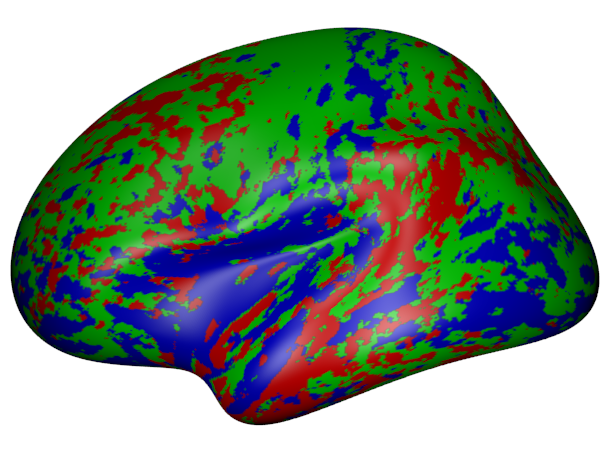
\includegraphics[width=\scalingFactorBrains\textwidth,trim=0 30 0 0]{figures/blend14_adniThavgFWHM0InithistCl3Pr0Ra1_VWDPMStd.png}}; 
    \node[inner sep=0] (label) at (0,1.5) {tAD - ADNI};
  \end{tikzpicture}
    \caption{}
      \label{fig:adniClust}
  \end{subfigure}
   \begin{subfigure}[b]{0.3\textwidth}
  \centering
  \begin{tikzpicture}[scale=\scalingFactor]
    \node[inner sep=0] (corr_text) at (0,0) {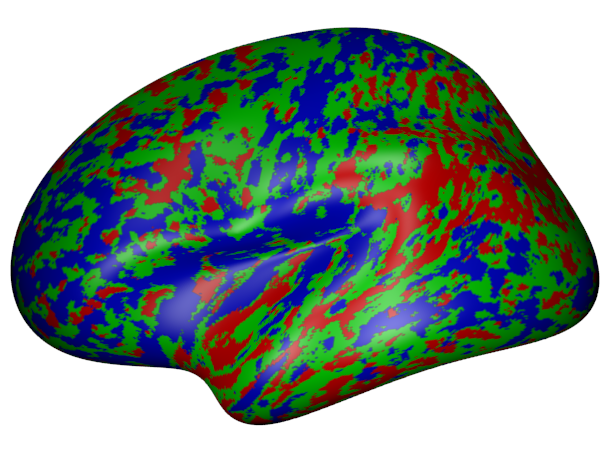
\includegraphics[width=\scalingFactorBrains\textwidth,trim=0 30 0 0]{figures/drcThavgFWHM0InithistCl3Pr0Ra1_VWDPMStdAD_blend24.png}};
    \node[inner sep=0] (label) at (0,1.5) {tAD - DRC dataset};
  \end{tikzpicture}
    \caption{}
      \label{fig:drcClustAD}
  \end{subfigure}
   \begin{subfigure}[b]{0.3\textwidth}
  \centering
  \begin{tikzpicture}[scale=\scalingFactor, every node/.style={scale=\scalingFactor}]
    \node[inner sep=0] (corr_text) at (0,0) {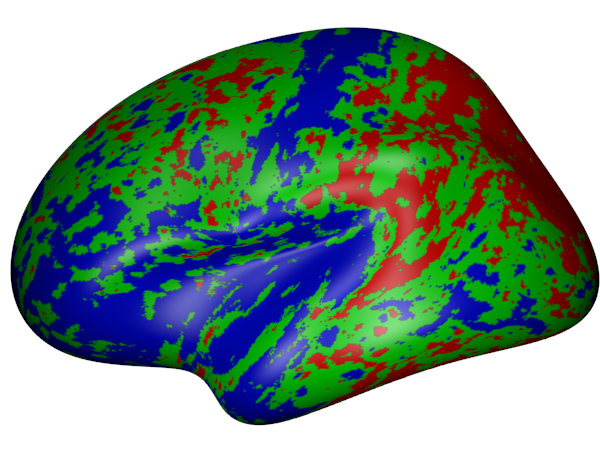
\includegraphics[width=\scalingFactorBrains\textwidth,trim=0 30 0 0]{figures/drcThavgFWHM0InithistCl3Pr0Ra1_VWDPMStdPCA_blend24.png}};
    \node[inner sep=0] (label) at (0,1.5) {PCA - DRC dataset};
  \end{tikzpicture}
    \caption{}
      \label{fig:drcClustPCA}
  \end{subfigure}
  
  %%%%%%%%%%%%%%%%%%%%%% trajectories %%%%%%%%%%%%%%%%%%%%%%%
  
    \begin{subfigure}[b]{0.3\textwidth}
    \centering
%     \vspace{-2em}
    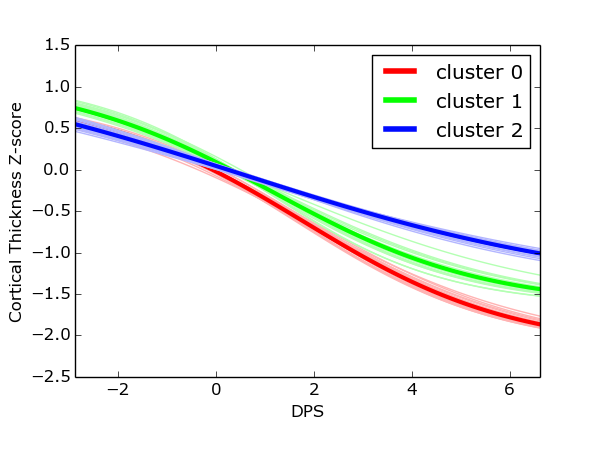
\includegraphics[width=\scalingFactorTraj\textwidth,trim=0 30 0 0]{figures/trajSamplesOneFig_adniThavgFWHM0InithistCl3Pr0Ra1_VWDPMStd.png}
    \caption{}
      \label{fig:adniTraj}
  \end{subfigure}
      \begin{subfigure}[b]{0.3\textwidth}
    \centering
%     \vspace{-2em}
    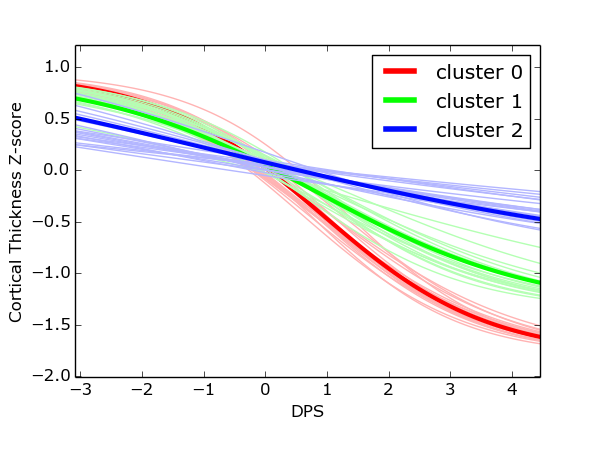
\includegraphics[width=\scalingFactorTraj\textwidth,trim=0 30 0 0]{figures/trajSamplesOneFig_drcThavgFWHM0InithistCl3Pr0Ra1_VWDPMStdAD.png}
    \caption{}
      \label{fig:drcTrajAD}
  \end{subfigure}
    \begin{subfigure}[b]{0.3\textwidth}
    \centering
%     \vspace{-2em}
    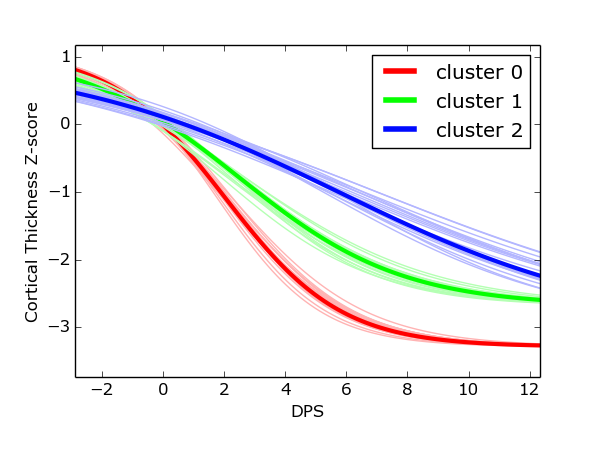
\includegraphics[width=\scalingFactorTraj\textwidth,trim=0 30 0 0]{figures/trajSamplesOneFig_drcThavgFWHM0InithistCl3Pr0Ra1_VWDPMStdPCA.png}
    \caption{}
      \label{fig:drcTrajPCA}
  \end{subfigure}
  
  \caption{(a) Clustering results on the ADNI data using our model, where each cluster is coloured according to the slope of its corresponding trajectory, from red (high slope suggesting very affected areas) to blue (low slope suggesting less affected areas). (d) The corresponding trajectories and samples from the posterior distribution of the trajectory  parameters for the three clusters in ADNI. The same analysis is shown also for (b, e) tAD subjects from the DRC cohort and (c, f) PCA subjects from the DRC cohort.}
  \label{fig:clustTrajAll}

\end{figure}

\subsection{Model Validation}

% motivation, i.e. what we wanted to test
We tested robustness of the model by performing 10-fold cross validation (CV) on ADNI. Our motivation was to test the following: (1) if similar spatial clustering is estimated at each fold, as quantified by Dice score overlap, (2) if the stages of the test subjects were consistent (i.e. were increasing for follow-up visits) and (3) if the stages of test subjects are clinically meaningful, by correlating them with cognitive tests such as Clinical Dementia Rating Scale - Sum of Boxes (CDRSOB), Alzheimer's Disease Assessment Scale - Cognitive (ADAS-COG), Mini-Mental State Examination (MMSE) and Rey Auditory and Verbal Learning Test (RAVLT).

% results 
Fig \ref{fig:ADNICVbrains} shows the clusters that were estimated at each fold from the training data only. Moreover, in Fig. \ref{fig:stagingConsist} we plot the estimated DPS (i.e. disease stage) of each subject from the test set against their age.

% conclusion
The results in Fig. \ref{fig:ADNICVbrains} prove that the model is robust in cross-validation, as the estimated clusters are all very similar across folds. The average Dice scores we obtained across all pairs of folds were 0.89, 0.89 and 0.90 for clusters 0, 1 and 2 respectively. Furthermore, 84\% of the subjects analysed show increased stages across their follow-up visits, proving that the estimated stages are mostly consistent. Finally, the stages of test subject correlate with clinical measures such as CDRSOB ($\rho = 0.41$, $p < 1e-66$), ADAS-COG ($\rho = 0.40$, $p < 1e-62$), MMSE ($\rho = 0.39$, $p < 1e-58$) and RAVLT ($\rho = 0.35$, $p < 1e-46$), demonstrating that the stages have clinical validity.

\newcommand{\outFoldADNICVbrains}{figures/crossvalid/adniThavgFWHM0Initk-meansCl3Pr0Ra1_VWDPMMean}

\newcommand{\trimModelValidTop}{150}

\begin{figure}[h]
    \centering
    
    \begin{subfigure}[b]{0.19\textwidth}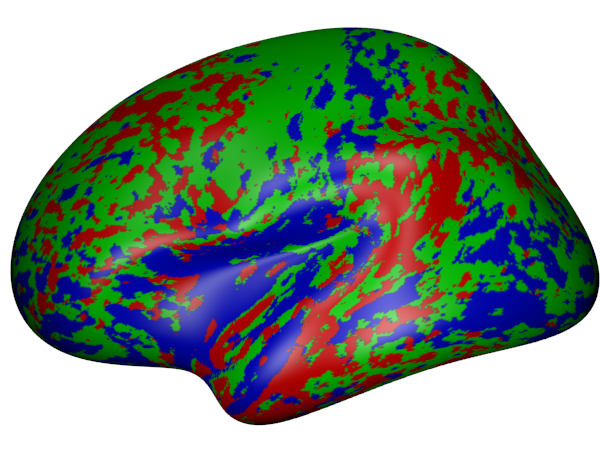
\includegraphics[width=\textwidth, trim=0 20 0 \trimModelValidTop]{\outFoldADNICVbrains/blend0.png}\end{subfigure}
    \begin{subfigure}[b]{0.19\textwidth}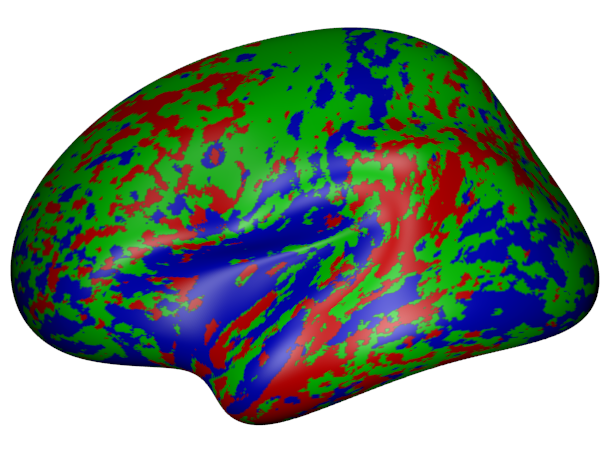
\includegraphics[width=\textwidth, trim=0 20 0 \trimModelValidTop]{\outFoldADNICVbrains/blend1.png}\end{subfigure}
    \begin{subfigure}[b]{0.19\textwidth}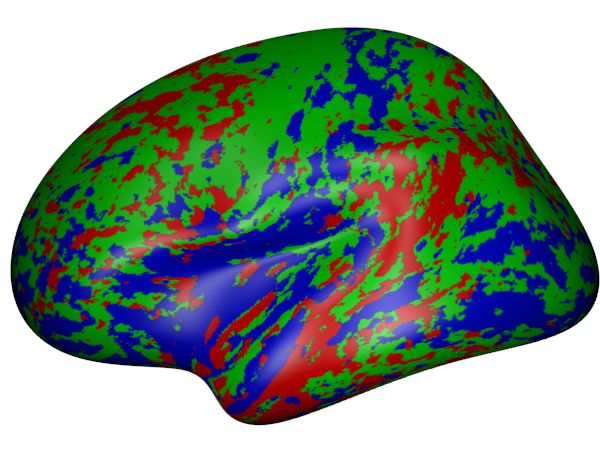
\includegraphics[width=\textwidth, trim=0 20 0 \trimModelValidTop]{\outFoldADNICVbrains/blend2.png}\end{subfigure}
    \begin{subfigure}[b]{0.19\textwidth}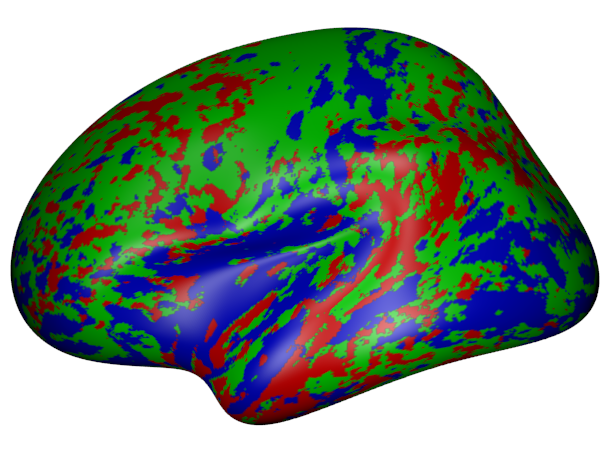
\includegraphics[width=\textwidth, trim=0 20 0 \trimModelValidTop]{\outFoldADNICVbrains/blend3.png}\end{subfigure}
    \begin{subfigure}[b]{0.19\textwidth}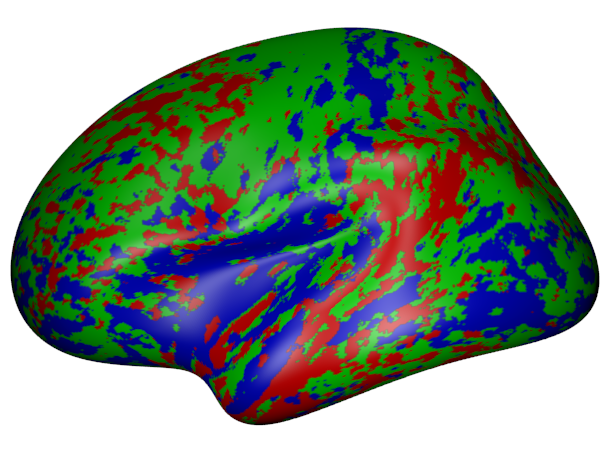
\includegraphics[width=\textwidth, trim=0 20 0 \trimModelValidTop]{\outFoldADNICVbrains/blend4.png}\end{subfigure}
    \begin{subfigure}[b]{0.19\textwidth}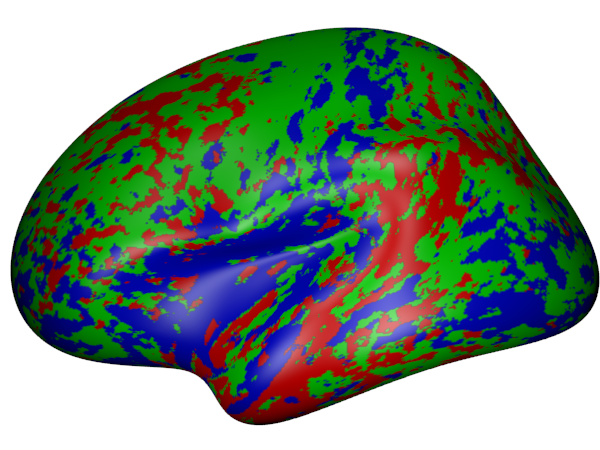
\includegraphics[width=\textwidth, trim=0 20 0 0]{\outFoldADNICVbrains/blend5.png}\end{subfigure}
    \begin{subfigure}[b]{0.19\textwidth}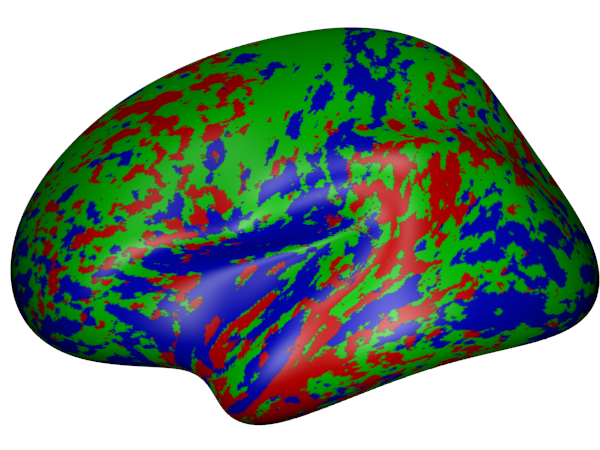
\includegraphics[width=\textwidth, trim=0 20 0 0]{\outFoldADNICVbrains/blend6.png}\end{subfigure}
    \begin{subfigure}[b]{0.19\textwidth}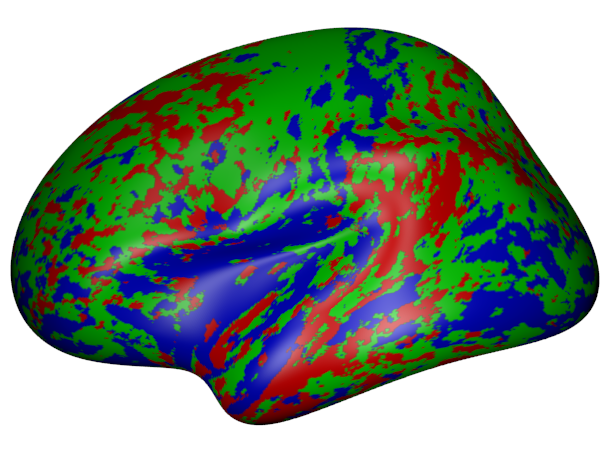
\includegraphics[width=\textwidth, trim=0 20 0 0]{\outFoldADNICVbrains/blend7.png}\end{subfigure}
    \begin{subfigure}[b]{0.19\textwidth}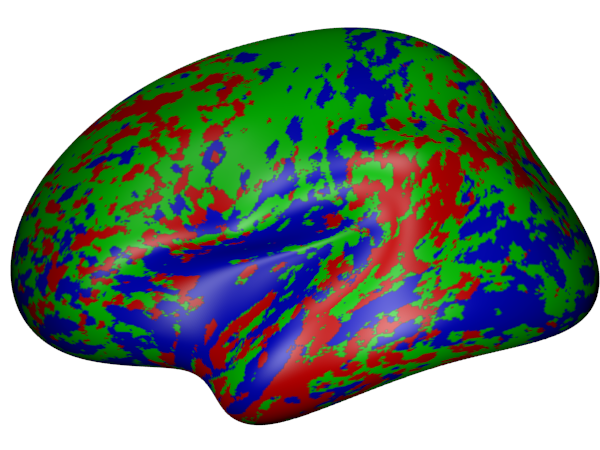
\includegraphics[width=\textwidth, trim=0 20 0 0]{\outFoldADNICVbrains/blend8.png}\end{subfigure}
    \begin{subfigure}[b]{0.19\textwidth}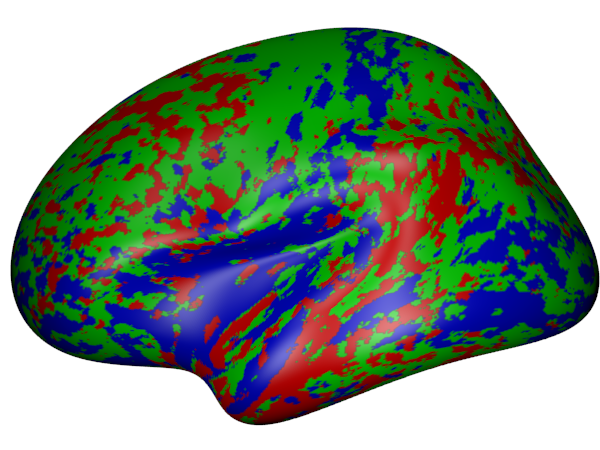
\includegraphics[width=\textwidth, trim=0 20 0 0]{\outFoldADNICVbrains/blend9.png}\end{subfigure}
    
    \caption{Clusters estimated for each of the 10 cross-validation folds in ADNI. As before, each cluster is coloured according to the slope of its corresponding trajectory, from red (high rate of atrophy) to blue (low rate of atrophy).}
    \label{fig:ADNICVbrains}
\end{figure}


\begin{figure}[h]
    \centering
    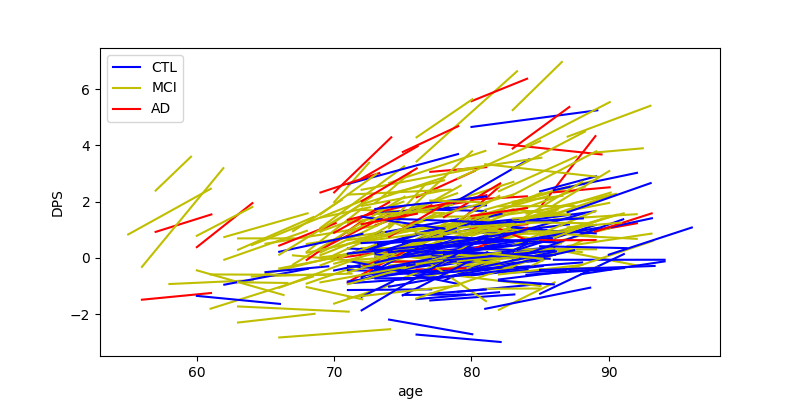
\includegraphics[width=0.7\textwidth, trim=0 10 0 100]{figures/crossvalid/stagingConsistWide_adniThavgFWHM0Initk-meansCl3Pr0Ra1_VWDPMMean.png}
    \caption{The disease progression score for each subject from the ADNI dataset estimated during 10-fold cross validation. Each line represents an individual $i$ with different visits $j$. Later visits generally have a higher corresponding stage.}
    \label{fig:stagingConsist}
\end{figure}

\section{Discussion}

% summary -> other types of data -> not regress against age -> disease progression space -> model worked ok -> stages better than with static ROIs
We presented a model of disease progression that clusters vertex-wise measures of cortical thickness based on similar temporal dynamics. The model highlights, for the first time, groups of cortical vertices that exhibit a similar temporal trajectory over the population. This provides a new way to parcellate the brain that is specific to the temporal trajectory of a particular disease. The model also finds the optimal temporal shift and progression speed for every subject. We applied the model to cortical thickness vertex-wise data from the ADNI and DRC cohorts. Our model found similar patterns of atrophy dynamics in the tAD subjects using the two independent datasets. Moreover, it also found different patterns of atrophy dynamics on two distinct diseases: tAD and PCA. 

% Limitations of the model
% a priori # of clust -> but can do BIC maximisation -> traj assumed sigmoidal -> but can use non-parametric curves -> Bias due to z-score normalisation - > susceptible to registration errors
The model has some limitations. First of all, we assumed that cluster trajectories follow sigmoidal shapes, which might not be the case for many types of biomarkers such as cortical thickness. Another limitation of the model is that it assumes all subjects follow the same disease progression pattern, which might not be the case in heterogeneous datasets such as ADNI or DRC. This can be a concern, as there might be a pattern of atrophy that occurs in a small set of subjects. Moreover, our cluster-based model might miss atrophy patterns that occur is very small regions. Furthermore, the data we analysed has been standardised with respect to controls, which assumes controls don't show any biomarker abnormalities.

% future work on technical improvements, motivated by the limitations mentioned before
There are several potential avenues of future research. While we only used the model for studying cortical thickness, one can also apply it to other types of data such as amyloid images or Jacobian compression maps. On the methodological side, the assumption of sigmoidal trajectories can be avoided using non-parametric curves such as Gaussian Processes. Another extension is to model different progression dynamics for distinct subgroups using unsupervised learning methods like the approach of \cite{young2015multiple}, or incorporate subject-specific deviations from the standard pattern of atrophy using a mixed-effects model.

% potential impact, clinical applications, work required to get there
Our approach can be used for accurately predicting and staging patients across the progression timeline of neurodegenerative diseases. This is promising for patient prognosis, as well as in clinical-trials for assessing efficacy of a putative treatment for slowing down the degeneration process.

\section{Acknowledgements}

This work was supported by the EPSRC Centre For Doctoral Training in Medical Imaging with grant EP/L016478/1. AE received a McDonald Fellowship from the Multiple Sclerosis International Federation (MSIF, www.msif.org), and the ECTRIMS - MAGNIMS Fellowship. ALY was supported through EPSRC grant EP/J020990/01. NPO and SG received funding from the EU Horizon 2020 research and innovation programme under grant agreement No 666992. SJC was supported by an Alzheimer’s Research UK Senior Research Fellowship and ESRC/NIHR (ES/L001810/1) and EPSRC (EP/M006093/1) grants. DCA's work on this topic has funding from the EU Horizon 2020 research and innovation programme under grant agreement No 666992, as well as EPSRC grants J020990, M006093 and M020533. Data collection and sharing for this project was funded by the Alzheimer's Disease Neuroimaging Initiative (ADNI) (National Institutes of Health Grant U01 AG024904) and DOD ADNI (Department of Defense award number W81XWH-12-2-0012). The Dementia Research Centre is an ARUK coordination center.


%
% ---- Bibliography ---- 
% USE HARVARD STANDARD

\bibliographystyle{unsrtnat}
\begin{thebibliography}{5}

\bibitem{jack2010hypothetical}
Jack, C.R., Knopman, D.S., Jagust, W.J., Shaw, L.M., Aisen, P.S., Weiner, M.W., Petersen, R.C. and Trojanowski, J.Q., 2010. Hypothetical model of dynamic biomarkers of the Alzheimer's pathological cascade. The Lancet Neurology, 9(1), pp.119-128.

\bibitem{bateman2012clinical}
Bateman, R.J., Xiong, C., Benzinger, T.L., Fagan, A.M., Goate, A., Fox, N.C., Marcus, D.S., Cairns, N.J., Xie, X., Blazey, T.M. and Holtzman, D.M., 2012. Clinical and biomarker changes in dominantly inherited Alzheimer's disease. New England Journal of Medicine, 367(9), pp.795-804.

\bibitem{richberg2015multi}
Schmidt-Richberg, A., Guerrero, R., Ledig, C., Molina-Abril, H., Frangi, A.F., Rueckert, D. and Alzheimers Disease Neuroimaging Initiative, 2015, June. Multi-stage Biomarker Models for Progression Estimation in Alzheimer’s Disease. In International Conference on Information Processing in Medical Imaging (pp. 387-398). Springer International Publishing.

\bibitem{fonteijn2012event}
Fonteijn, H.M., Modat, M., Clarkson, M.J., Barnes, J., Lehmann, M., Hobbs, N.Z., Scahill, R.I., Tabrizi, S.J., Ourselin, S., Fox, N.C. and Alexander, D.C., 2012. An event-based model for disease progression and its application in familial Alzheimer's disease and Huntington's disease. NeuroImage, 60(3), pp.1880-1889.

\bibitem {jedynak2012}
Jedynak, B.M., Lang, A., Liu, B., Katz, E., Zhang, Y., Wyman, B.T., Raunig, D., Jedynak, C.P., Caffo, B., Prince, J.L. and Alzheimer's Disease Neuroimaging Initiative, 2012. A computational neurodegenerative disease progression score: method and results with the Alzheimer's Disease Neuroimaging Initiative cohort. Neuroimage, 63(3), pp.1478-1486.

\bibitem{donohue2014estimating}
Donohue, M.C., Jacqmin-Gadda, H., Le Goff, M., Thomas, R.G., Raman, R., Gamst, A.C., Beckett, L.A., Jack, C.R., Weiner, M.W., Dartigues, J.F. and Aisen, P.S., 2014. Estimating long-term multivariate progression from short-term data. Alzheimer's \& Dementia, 10(5), pp.S400-S410.

\bibitem{schiratti2015mixed}
Schiratti, J.B., Allassonniere, S., Routier, A., Colliot, O., Durrleman, S. and Alzheimers Disease Neuroimaging Initiative, 2015, June. A mixed-effects model with time reparametrization for longitudinal univariate manifold-valued data. In International Conference on Information Processing in Medical Imaging (pp. 564-575). Springer International Publishing.

\bibitem{bilgel2016multivariate}
Bilgel, M., Prince, J.L., Wong, D.F., Resnick, S.M. and Jedynak, B.M., 2016. A multivariate nonlinear mixed effects model for longitudinal image analysis: Application to amyloid imaging. NeuroImage, 134, pp.658-670.

\bibitem{seeley2009neurodegenerative}
Seeley, W.W., Crawford, R.K., Zhou, J., Miller, B.L. and Greicius, M.D., 2009. Neurodegenerative diseases target large-scale human brain networks. Neuron, 62(1), pp.42-52.

% \bibitem{bishop2006}
% Bishop, C.M., 2006. Pattern recognition. Machine Learning, 128.

\bibitem{reuter2012longitudinal}
Reuter, M., Schmansky, N.J., Rosas, H.D. and Fischl, B., 2012. Within-subject template estimation for unbiased longitudinal image analysis. Neuroimage, 61(4), pp.1402-1418.

% \bibitem{reuter2010inverse}
% Reuter, M., Rosas, H.D. and Fischl, B., 2010. Highly accurate inverse consistent registration: a robust approach. Neuroimage, 53(4), pp.1181-1196.

\bibitem{dickerson2009cortical}
Dickerson, B.C., Bakkour, A., Salat, D.H., Feczko, E., Pacheco, J., Greve, D.N., Grodstein, F., Wright, C.I., Blacker, D., Rosas, H.D. and Sperling, R.A., 2009. The cortical signature of Alzheimer's disease: regionally specific cortical thinning relates to symptom severity in very mild to mild AD dementia and is detectable in asymptomatic amyloid-positive individuals. Cerebral cortex, 19(3), pp.497-510.

% \bibitem{thompson2001cortical}
% Thompson, P.M., Mega, M.S., Woods, R.P., Zoumalan, C.I., Lindshield, C.J., Blanton, R.E., Moussai, J., Holmes, C.J., Cummings, J.L. and Toga, A.W., 2001. Cortical change in Alzheimer's disease detected with a disease-specific population-based brain atlas. Cerebral Cortex, 11(1), pp.1-16.

\bibitem{crutch2012posterior}
Crutch, S.J., Lehmann, M., Schott, J.M., Rabinovici, G.D., Rossor, M.N. and Fox, N.C., 2012. Posterior cortical atrophy. The Lancet Neurology, 11(2), pp.170-178.

\bibitem{young2015multiple}
Young, A.L., Oxtoby, N.P., Huang, J., Marinescu, R.V., Daga, P., Cash, D.M., Fox, N.C., Ourselin, S., Schott, J.M., Alexander, D.C. and Alzheimers Disease Neuroimaging Initiative, 2015, June. Multiple Orderings of Events in Disease Progression. In International Conference on Information Processing in Medical Imaging (pp. 711-722). Springer International Publishing.

\end{thebibliography}

\clearpage

\end{document}

